\documentclass[12pt,t]{beamer}
\usepackage{graphicx}
\setbeameroption{hide notes}
\setbeamertemplate{note page}[plain]
\usepackage{listings}

% get rid of junk
\usetheme{default}
\beamertemplatenavigationsymbolsempty
\hypersetup{pdfpagemode=UseNone} % don't show bookmarks on initial view


% font
\usepackage{fontspec}
\setsansfont
  [ ExternalLocation = Stuff/fonts/ ,
    UprightFont = *-regular , 
    BoldFont = *-bold ,
    ItalicFont = *-italic ,
    BoldItalicFont = *-bolditalic ]{texgyreheros}
\setbeamerfont{note page}{family*=pplx,size=\footnotesize} % Palatino for notes
% "TeX Gyre Heros can be used as a replacement for Helvetica"
% I've placed them in ../fonts/; alternatively you can install them
% permanently on your system as follows:
%     Download http://www.gust.org.pl/projects/e-foundry/tex-gyre/heros/qhv2.004otf.zip
%     In Unix, unzip it into ~/.fonts
%     In Mac, unzip it, double-click the .otf files, and install using "FontBook"

% named colors
\definecolor{offwhite}{RGB}{255,250,240}
\definecolor{gray}{RGB}{155,155,155}

\ifx\notescolors\undefined % slides
  \definecolor{foreground}{RGB}{255,255,255}
  \definecolor{background}{RGB}{24,24,24}
  \definecolor{title}{RGB}{107,174,214}
  \definecolor{subtitle}{RGB}{102,255,204}
  \definecolor{hilit}{RGB}{102,255,204}
  \definecolor{vhilit}{RGB}{255,111,207}
  \definecolor{lolit}{RGB}{155,155,155}
\else % notes
  \definecolor{background}{RGB}{255,255,255}
  \definecolor{foreground}{RGB}{24,24,24}
  \definecolor{title}{RGB}{27,94,134}
  \definecolor{subtitle}{RGB}{22,175,124}
  \definecolor{hilit}{RGB}{122,0,128}
  \definecolor{vhilit}{RGB}{255,0,128}
  \definecolor{lolit}{RGB}{95,95,95}
\fi
\definecolor{nhilit}{RGB}{128,0,128}  % hilit color in notes
\definecolor{nvhilit}{RGB}{255,0,128} % vhilit for notes

\newcommand{\hilit}{\color{hilit}}
\newcommand{\vhilit}{\color{vhilit}}
\newcommand{\nhilit}{\color{nhilit}}
\newcommand{\nvhilit}{\color{nvhilit}}
\newcommand{\lolit}{\color{lolit}}

% use those colors
\setbeamercolor{titlelike}{fg=title}
\setbeamercolor{subtitle}{fg=subtitle}
\setbeamercolor{institute}{fg=lolit}
\setbeamercolor{normal text}{fg=foreground,bg=background}
\setbeamercolor{item}{fg=foreground} % color of bullets
\setbeamercolor{subitem}{fg=lolit}
\setbeamercolor{itemize/enumerate subbody}{fg=lolit}
\setbeamertemplate{itemize subitem}{{\textendash}}
\setbeamerfont{itemize/enumerate subbody}{size=\footnotesize}
\setbeamerfont{itemize/enumerate subitem}{size=\footnotesize}

% page number
\setbeamertemplate{footline}{%
    \raisebox{5pt}{\makebox[\paperwidth]{\hfill\makebox[20pt]{\lolit
          \scriptsize\insertframenumber}}}\hspace*{5pt}}

% add a bit of space at the top of the notes page
\addtobeamertemplate{note page}{\setlength{\parskip}{12pt}}

% default link color
\hypersetup{colorlinks, urlcolor={hilit}}

\ifx\notescolors\undefined % slides
  % set up listing environment
  \lstset{language=bash,
          basicstyle=\ttfamily\scriptsize,
          frame=single,
          commentstyle=,
          backgroundcolor=\color{darkgray},
          showspaces=false,
          showstringspaces=false
          }
\else % notes
  \lstset{language=bash,
          basicstyle=\ttfamily\scriptsize,
          frame=single,
          commentstyle=,
          backgroundcolor=\color{offwhite},
          showspaces=false,
          showstringspaces=false
          }
\fi

% a few macros
\newcommand{\bi}{\begin{itemize}}
\newcommand{\bbi}{\vspace{24pt} \begin{itemize} \itemsep8pt}
\newcommand{\ei}{\end{itemize}}
\newcommand{\ig}{\includegraphics}
\newcommand{\subt}[1]{{\footnotesize \color{subtitle} {#1}}}
\newcommand{\ttsm}{\tt \small}
\newcommand{\ttfn}{\tt \footnotesize}
\newcommand{\figh}[2]{\centerline{\includegraphics[height=#2\textheight]{#1}}}
\newcommand{\figw}[2]{\centerline{\includegraphics[width=#2\textwidth]{#1}}}




\title{Salvaging a genetics project}
\subtitle{Identifying and correcting \\
  sample mix-ups in genetic data}
\author{\href{http://kbroman.org}{Karl Broman}}
\institute{Biostatistics \& Medical Informatics, UW{\textendash}Madison}
\date{\href{http://kbroman.org}{\tt \scriptsize \color{foreground} kbroman.org}
\\[-4pt]
\href{http://github.com/kbroman}{\tt \scriptsize \color{foreground} github.com/kbroman}
\\[-4pt]
\href{https://twitter.com/kwbroman}{\tt \scriptsize \color{foreground} @kwbroman}
}


\begin{document}

{
\setbeamertemplate{footline}{} % no page number here
\frame{
  \titlepage

\vspace{-40pt}

\centerline{\href{http://bit.ly/berkeley2017}{\tt \scriptsize bit.ly/berkeley2017}}

\vspace{-7mm}
\hfill 
\includegraphics[height=6mm]{Figs/cc-zero.png}

\note{
}
} }



\begin{frame}[c]{}

\vspace*{-1mm} \hspace*{-2mm}
\figw{Figs/inbredmice.jpg}{1.2}

\note{
I'll start with a bit of background.

I focus on genetics problems, and particularly on mouse genetics.

I think these are SWR mice; the photo is from David Threadgill.
}

\end{frame}


\begin{frame}{}

\vspace*{18mm}

\centerline{
\begin{minipage}[t]{50mm}
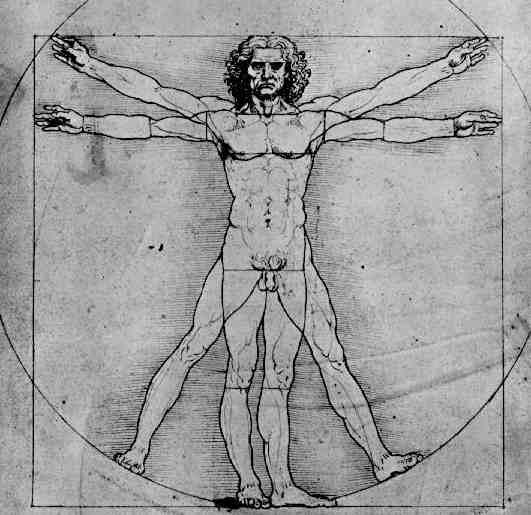
\includegraphics[height=50mm]{Figs/da-vinci-man.jpg}
\end{minipage}
\hspace{15mm}
\begin{minipage}[t]{50mm}
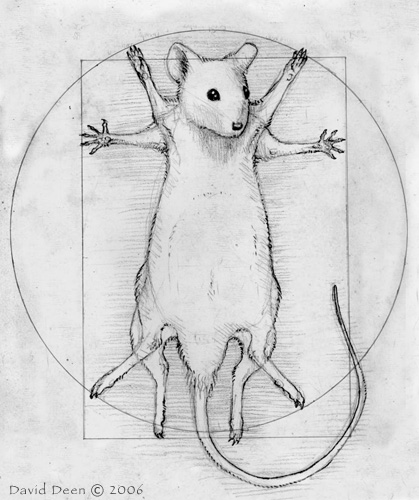
\includegraphics[height=50mm]{Figs/vitruvian_mouse.jpg}
\hspace{5mm}
\href{http://daviddeen.com}{\scriptsize \lolit \tt daviddeen.com}
\end{minipage}
}


\note{
Mice are not humans, but you can learn a great deal about human
biology and disease from mice.

The figure on the right is from David Deen.
}

\end{frame}


\begin{frame}[c]{Intercross}

\figh{Figs/intercross.pdf}{0.9}

\note{
  I've mostly focused on simple crosses between two inbred strains.

  Say strain P$_1$ has low blood pressure and P$_2$ has high blood
  pressure. We cross the two strains to get the F$_1$ hybrid, and then
  intercross F$_1$ siblings to get a large set of F$_2$
  individuals.

  The F$_2$ mice may inherit a P$_1$ or P$_2$ chromosome
  intact, but generally their chromosomes are a mosaic of the two
  parental chromosomes as a result of recombination at meiosis.  The
  points of exchange are called crossovers or recombination events.

  At any one autosomal locus, the F$_2$ individuals will have genotype
  BB, BR, or RR. We'd generate many such mice and then determine their
  genotype along chromosomes as well as measure their phenotype (e.g.,
  blood pressure). The simplest analyis is to look for genomic regions
  where genotype is associated with phenotype.
}
\end{frame}


\begin{frame}[c]{Data}

\hspace{0mm}

\figw{Figs/data_fig.png}{1.15}

\note{
  The data consist of genotypes at a set of markers across the genome,
  plus some quantitative phenotype for each mouse. The goal is to
  identify regions of the genome where the genotype is associated with
  the phenotype.
}
\end{frame}


\begin{frame}[c]{QTL mapping}

\vspace{5mm}
\only<1 | handout 0>{\figh{Figs/lodcurve_insulin.pdf}{0.85}}
\only<2>{\figh{Figs/lodcurve_insulin_with_effects.pdf}{0.85}}

\note{
  Our goal is to identify quantitative trait loci (QTL): regions of
  the genome for which genotype is associated with the phenotype.

  The basic analysis is to consider each locus, one at a time, split
  the mice into the three genotype groups, and perform analysis of
  variance.

  We then plot a test statistic that indicates the strength of the
  genotype-phenotype association.  For historical reasons, we
  calculate a LOD score as the test statistic: the log$_{10}$
  likelihood ratio comparing the hypothesis that there's a QTL at that
  position to the null hypothesis of no QTL anywhere.

  Large LOD scores indicate evidence for QTL and correspond to there
  being a difference in the phenotype average for the three genotype
  groups.
}
\end{frame}




\begin{frame}[c]{Attie project}


{\hilit
$\sim$500 B6 $\times$ BTBR intercross mice, all ob/ob }

\vspace{6pt}

\begin{itemize}
\itemsep12pt
\item Genotypes at 2057 SNPs (Affymetrix arrays)

\item Gene expression in six tissues (Agilent arrays)

  \begin{itemize}
    \item adipose
    \item gastrocnemius muscle
    \item hypothalamus
    \item pancreatic islets
    \item kidney
    \item liver
  \end{itemize}

\item Numerous clinical phenotypes
  \begin{itemize}
    \item[] (e.g., body weight, insulin and glucose levels)
  \end{itemize}

\end{itemize}

\note{}

\end{frame}




\begin{frame}[c]{Sex and the X chr}
\figh{Figs/xchr_fig.pdf}{0.85}
\note{}
\end{frame}


\begin{frame}[c]{Genotype mix-ups}
\figw{Figs/plate_errors.pdf}{1.1}
\note{}
\end{frame}


\begin{frame}[c]{Sex and the X chr}
\figh{Figs/xchr_fig.pdf}{0.85}
\note{}
\end{frame}


\begin{frame}[c]{Strong eQTL}
\only<1|handout 0>{\figh{Figs/eqtl_lod_1.pdf}{0.85}}
\only<2>{\figh{Figs/eqtl_lod_2.pdf}{0.85}}
\note{}
\end{frame}




\begin{frame}[c]{E vs G}
\only<1|handout 0>{\figh{Figs/gve1a.pdf}{0.85}}
\only<2>{\figh{Figs/gve1b.pdf}{0.85}}
\note{}
\end{frame}


\begin{frame}[c]{kNN classifier}
\figh{Figs/gve1c.pdf}{0.85}
\note{}
\end{frame}


\begin{frame}[c]{E vs G}
\only<1|handout 0>{\figh{Figs/gve3a.pdf}{0.85}}
\only<2>{\figh{Figs/gve3b.pdf}{0.85}}
\note{}
\end{frame}


\begin{frame}[c]{E vs G}
\only<1|handout 0>{\figh{Figs/gve2a.pdf}{0.85}}
\only<2>{\figh{Figs/gve2b.pdf}{0.85}}
\note{}
\end{frame}


\begin{frame}[c]{Basic scheme}
\only<1|handout 0>{\figh{Figs/gve_scheme_1.pdf}{0.85}}
\only<2|handout 0>{\figh{Figs/gve_scheme_2.pdf}{0.85}}
\only<3|handout 0>{\figh{Figs/gve_scheme_3.pdf}{0.85}}
\only<4>{\figh{Figs/gve_scheme_4.pdf}{0.85}}
\note{}
\end{frame}

\begin{frame}[c]{Prop'n mismatches}
\figh{Figs/distmatall.png}{0.85}
\note{}
\end{frame}

\begin{frame}[c]{Prop'n mismatches}
\figh{Figs/distmat001.pdf}{0.85}
\note{}
\end{frame}

\begin{frame}[c]{Prop'n mismatches}
\figh{Figs/distmat201.pdf}{0.85}
\note{}
\end{frame}


\begin{frame}[c]{Prop'n mismatches}
\figh{Figs/gve_dist.pdf}{0.85}
\note{}
\end{frame}


\begin{frame}[c]{Decisions}
\figh{Figs/gve_dist_byrow_left.pdf}{0.85}
\note{}
\end{frame}


\begin{frame}[c]{Genotype mix-ups}
\figh{Figs/plate_errors.pdf}{0.85}
\note{}
\end{frame}


\begin{frame}[c]{Plate 1631}
\figh{Figs/plate_errors_1631.png}{0.65}
\note{}
\end{frame}

\begin{frame}[c]{Plates 1632 and 1630}
\figh{Figs/plate_errors_1632_n_1630.png}{0.85}
\note{}
\end{frame}

\begin{frame}[c]{Plate 1630}
\figh{Figs/plate_errors_1630.png}{0.65}
\note{}
\end{frame}


\begin{frame}[c]{E vs E}
\figh{Figs/eve_1.pdf}{0.85}
\note{}
\end{frame}


\begin{frame}[c]{E vs E}
\figh{Figs/eve_2.pdf}{0.85}
\note{}
\end{frame}


\begin{frame}[c]{E vs E}
\figh{Figs/eve_3.jpg}{0.85}
\note{}
\end{frame}


\begin{frame}[c]{E vs E}
\figh{Figs/eve_3b.pdf}{0.85}
\note{}
\end{frame}


\begin{frame}[c]{E vs E}
\figh{Figs/eve_3c.pdf}{0.85}
\note{}
\end{frame}


\begin{frame}[c]{E vs E}
\figh{Figs/eve_3d.pdf}{0.85}
\note{}
\end{frame}


\begin{frame}[c]{E vs E}
\figh{Figs/eve_4.pdf}{0.85}
\note{}
\end{frame}


\begin{frame}[c]{E vs E}
\figh{Figs/eve_5.pdf}{0.85}
\note{}
\end{frame}


\begin{frame}[c]{E vs E}
\figh{Figs/eve_6.pdf}{0.85}
\note{}
\end{frame}


\begin{frame}[c]{E vs E}
\figh{Figs/eve_7.pdf}{0.85}
\note{}
\end{frame}


\begin{frame}[c]{E vs E}
\figh{Figs/eve_8.pdf}{0.85}
\note{}
\end{frame}


\begin{frame}[c]{E vs E}
\figh{Figs/eve_9.pdf}{0.85}
\note{}
\end{frame}


\begin{frame}[c]{E vs E}
\figh{Figs/eve_10.pdf}{0.85}
\note{}
\end{frame}


\begin{frame}[c]{E vs E}
\figh{Figs/eve_11.pdf}{0.85}
\note{}
\end{frame}

\begin{frame}[c]{Expression mix-ups}
\figh{Figs/expr_swaps.pdf}{0.85}
\note{}
\end{frame}

\begin{frame}[c]{Insulin QTL}
\figh{Figs/insulin_lod.pdf}{0.85}
\note{}
\end{frame}


\begin{frame}[c]{Strong eQTL}
\figh{Figs/eqtl_lod_3.pdf}{0.85}
\note{}
\end{frame}


\begin{frame}[c]{Summary}


\small
\begin{itemize}
\itemsep3pt

\item Sample mix-ups happen


\item With eQTL data, we can both identify and {\hilit correct} mix-ups

\item There is great value in having expression on multiple tissues

\item The general idea here has wide application for high-throughput data

\item \href{https://www.ncbi.nlm.nih.gov/pubmed/26290572}{Broman et
  al. (2015) G3 5:2177-2186} \\
\href{http://doi.org/10.1534/g3.115.019778}{doi: 10.1534/g3.115.019778}

\item Related work:

\begin{itemize}
\item Westra et al. (2011) Bioinformatics 27:2104--2111
\item Schadt et al. (2012) Nat Genet 44:603--608
\item Ekstr{\o}m and Feenstra (2012) Stat Appl Genet Mol Biol
  3:Article 13
\item Lynch et al. (2012) PLoS ONE 7:e41815
\end{itemize}

\end{itemize}
\note{}
\end{frame}



\begin{frame}[c]{Lessons}

\small

\begin{itemize}
\itemsep8pt

\item Don't fully trust anyone
\begin{itemize}
\item Including yourself
\end{itemize}

\item Make lots of plots
\begin{itemize}
\item Don't rely on summary statistics, like LOD scores
\item Look at responses on the original scale
\end{itemize}

\item Follow up all aberrations

\item Take your time with data cleaning
\begin{itemize}
\item A month, two months, a year?
\end{itemize}

\item If you have big rectangles whose rows correspond, \\
  check that they {\hilit actually} correspond

\end{itemize}
\note{}
\end{frame}


\begin{frame}[c]{E vs G}

\only<1>{transformed scale}
\only<2>{original scale}

 \vspace{5mm}

\only<1>{\figh{Figs/gve1a_nqrank.pdf}{0.65}}
\only<2>{\figh{Figs/gve1a.pdf}{0.65}}

\note{}
\end{frame}



\begin{frame}[c]{Lessons}

\small

\begin{itemize}
\itemsep8pt

\item Don't fully trust anyone
\begin{itemize}
\item Including yourself
\end{itemize}

\item Make lots of plots
\begin{itemize}
\item Don't rely on summary statistics, like LOD scores
\item Look at responses on the original scale
\end{itemize}

\item Follow up all aberrations

\item Take your time with data cleaning
\begin{itemize}
\item A month, two months, a year?
\end{itemize}

\item If you have big rectangles whose rows correspond, \\
  check that they {\hilit actually} correspond

\end{itemize}
\note{}
\end{frame}



\begin{frame}[c]{Acknowledgments}

\setlength{\tabcolsep}{2mm}
{\footnotesize
\begin{tabular}{lll}
Alan Attie&&
{\lolit Biochemistry, UW--Madison} \\
Mark Keller &&
\\[10pt]

Brian Yandell &&
{\lolit Statistics and Horticulture, UW--Madison} \\[10pt]

Christina Kendziorski &&
{\lolit Biostat \& Medical Info, UW--Madison} \\
Aimee Teo Broman && \\[10pt]

Eric Schadt &&
{\lolit Mount Sinai} \\[10pt]

Danielle Greenawalt &&
{\lolit Merck \& Co., Inc.} \\
Amit Kulkarni && \\[10pt]

\'Saunak Sen &&
{\lolit UT-Memphis} \\[20pt]

\multicolumn{3}{l}{\hilit NIH: \lolit R01 GM074244, R01 DK066369}


\end{tabular}
}

\note{}
\end{frame}





\begin{frame}[c]{}

\large

\vspace*{10mm}
Slides: \href{http://bit.ly/berkeley2017}{\tt bit.ly/berkeley2017}

\vspace*{-5mm}
\hspace{90mm} 
\includegraphics[height=5mm]{Figs/cc-zero.png}

\vspace{2mm}

\href{http://kbroman.org}{\tt kbroman.org}

\vspace{2mm}

\href{https://github.com/kbroman}{\tt github.com/kbroman}

\vspace{2mm}

\href{https://twitter.com/kwbroman}{\tt @kwbroman}

\note{
  Here's where you can find me, as well as the slides for this talk.
}
\end{frame}



\begin{frame}[c]{Decisions}
\figh{Figs/gve_dist_byrow.pdf}{0.85}
\note{}
\end{frame}

\end{document}
